\documentclass[10pt]{article}
    \usepackage{graphicx}
    \usepackage{float}
    \title{Temperature Changes in Key West, Florida for the 20th century}
    \author{Yuchen Yang}
    \date{Oct. 2019}
\begin{document}
  \maketitle

  \begin{abstract}
  This report uses data from Key West, Florida as example, and explores the way to calculate p-value for sucessive years' temperature changes.
  \end{abstract}

  \section{Method}
    \textbf{greatestAre temperatures of one year significantly correlated with the next year (successive years), across years in a given location?} Standard p-value calculated for a correlation coefficient is not suitable to answer this question(not independent). Implementing the temperature data in Key West, Florida for the 20th century, the correlation coefficient is calculated and compared with a distribution of 10,000 randomly generated time-series correlations. The alternative and appropriate p-value was calculated by dividing the number of random sample correlations larger than the real value of West Key by the entire sample size, which is 10,000.

  \section{Result}
    \begin{figure}[H]
    \centering
    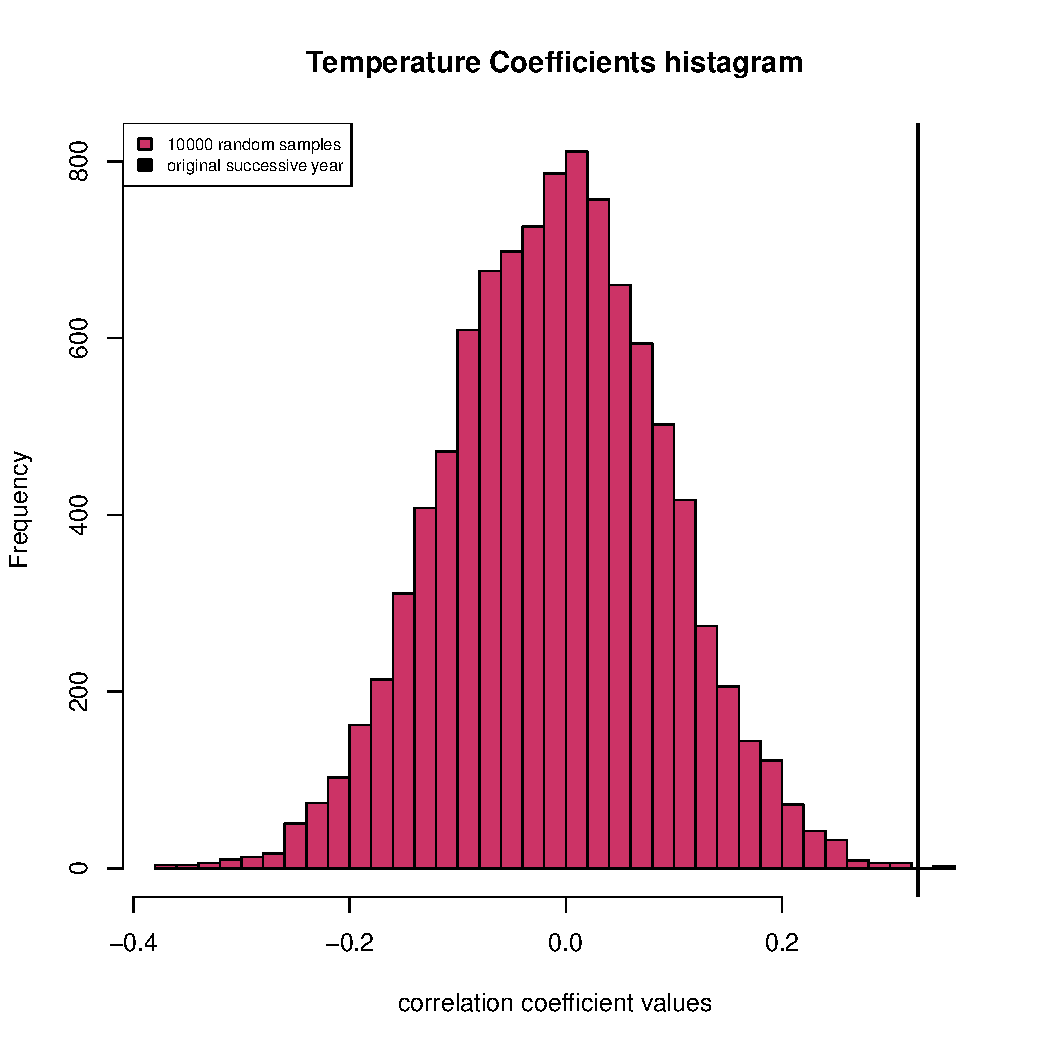
\includegraphics[width=0.90\textwidth]{../Results/TAutoCorr_graph.pdf}
    \caption{Temperature Coefficient Compared between Successive Years and Rondom Years in Key West, Florida from 1901-2000.}
    \end{figure}

    Figure above shows that the dataset for West Key, Florida has a correlation coefficients of $~0.33$ betweem successive years, which was calculated using $cor()$ in R. Only 4 correlation coefficient values from the 10,000-entry random sample set are greater than that, resulting a p-value of $0.0004$. This means it is extremely unlikely that the result is caused by chance, and can potentially indicate that one year's temperature is indicative of the subsequent year's.

\end{document}
